\section{¿Cómo analizamos las \textit{misconceptions}?}

Tras la lectura de la bibliografía de referencia, nos quedó claro que había dos caminos que podíamos recorrer para la recolección de información. Una opción era realizar entrevistas personales acompañadas por alguna actividad extra (por ejemplo dibujos, historias, etc). Esta alternativa nos pareció muy interesante: por un lado, da lugar a que los chicos se explayen libremente sobre sus pensamientos e ideas y, al mismo tiempo, nos permite un \textit{feedback} directo con ellos para poder repreguntar y entender a fondo sus respuestas.

Sin embargo, en el contexto de pandemia que estamos atravesando, las clases se estuvieron llevando a cabo en una modalidad mixta: presencial y online. Al mismo tiempo, la impredecibilidad de la situación no permitió saber a ciencia cierta cómo sería el futuro de las mismas. Por este motivo, encontramos que realizar una actividad presencial con los chicos era muy complicado en este momento, y resultaba una apuesta más segura el organizar una actividad asincrónica. Esta actividad podía ser regulada por un docente en los tiempos que él o ella considerase adecuados, y completada por los alumnos y alumnas ya sea en su casa o en la escuela.

Este tipo de actividad coincide con el otro camino que relevamos en la lectura de la bibliografía de referencia: un cuestionario con opciones para completar. Como una solución de compromiso con el camino descrito anteriormente, agregaremos la posibilidad de elaborar una respuesta propia en algunas preguntas en las que nos interesa que los chicos puedan explayarse o exponer sus ideas más libremente.

Este cuestionario se realizó en la plataforma \textit{Google Forms} para poder almacenar automáticamente las respuestas a las preguntas en un archivo de \textit{Google Spreadsheet} y poder analizar posteriormente la información de manera sistemática y práctica.

\section{¿Qué \textit{misconceptions} queremos analizar?}
\subsection{¿Qué es relevante para los chicos?}

Para empezar, nos propusimos pensar qué \textit{misconceptions} podíamos analizar, es decir, sobre qué temas íbamos a indagar.

Para obtener información relevante necesitamos captar el interés de los chicos y chicas. Para eso, los temas sobre los que les preguntemos tienen que ser no solo conocidos por ellos, sino también ser parte fundamental de su día a día. Tienen que ser temáticas que les interesen y sobre las que quieran detenerse a pensar o compartir su conocimiento al respecto.

Al intentar responder a esta pregunta, nos encontramos con el primer problema: por pertenecer a diferentes generaciones y no estar en contacto directo con chicos y chicas de 10 años, no estábamos muy seguros de cuáles son los temas con los que ellos y ellas están más en contacto. ¿Son consumidores ávidos de Netflix? ¿Utilizan solo YouTube? ¿Siguen usando Facebook? ¿E Instagram?

Para acercarnos a su realidad, pedimos ayuda a los referentes pedagógicos de la Fundación Sadosky que trabajan para el Plan Ceibal para que nos informaran acerca de los consumos informáticos que los chicos realizan hoy en día.

Nos enteramos de que la red social más ampliamente utilizada es TikTok, de la no solo son usuarios sino también en gran medida creadores de contenidos. Otras redes sociales, tales como Instagram o Facebook, son utilizadas para poder iniciar sesión en TikTok, o bien para ver \textit{live streaming} propios de esas plataformas.

Otro consumo instalado es WhatsApp, elegido mayoritariamente como medio de comunicación entre amigos y familia, y con la pandemia, también con la escuela.

En este rango de edad, los chicos y chicas eligen YouTube por sobre Netflix, siendo tanto consumidores como, en menor medida, creadores de contenido. De todas formas, están ampliamente familiarizados con ambas plataformas. Algunos otros utilizan también Twitch, una plataforma que permite realizar transmisiones en vivo.

El dispositivo por excelencia es el celular, todos tienen uno o tienen acceso a uno y saben cómo utilizarlo.

\section{Nuestra elección de \textit{misconceptions} a investigar}

Contando con esta información, elegimos algunos temas en los que nos interesa investigar si existen \textit{misconceptions} y, de haberlas, cuáles son. A continuación, detallamos cada uno de los temas escogidos.

\subsection{Dónde se almacenan los videos de YouTube}

En YouTube se suben aproximadamente 500 horas de contenido por minuto. Esta cantidad descomunal de datos es difícil de imaginar o cuantificar, incluso para nosotros, los adultos.  Y si bien los chicos y chicas son usuarios habituales de esta plataforma y están acostumbrados a utilizarla diariamente, queremos indagar si alguna vez habían pensado en este aspecto de YouTube.

¿Cuántos videos hay en YouTube? ¿Cuánto espacio ocupan? ¿En dónde se almacenan físicamente? ¿Se encuentran almacenados en un único lugar centralizado o de manera distribuida? Para poder despertarles algunas de estas preguntas y conocer cuales son sus concepciones al respecto, agregamos al cuestionario la siguiente pregunta disparadora: \textit{¿Dónde se almacenan los videos que están en YouTube?}

\subsection{De qué manera se comparte una foto por WhatsApp}

En el relevamiento de consumos tecnológicos pudimos conocer que WhatsApp es el medio de comunicación por excelencia. Desde edades cada vez más tempranas, los niños y niñas están familiarizados con mandar mensajes, fotos y archivos, y hacer videollamadas utilizando esta aplicación. 

Al enviar datos a través de WhatsApp, por ejemplo una foto o un archivo, se crea una copia en el teléfono de la o las personas que la reciben. Pero, ¿saben los chicos esto?

Este tema nos parece muy importante ya que es relevante para entender sobre la propiedad y privacidad de nuestros datos en Internet. El contar con este conocimiento hace posible tomar decisiones informadas al compartir información en línea.

Estas son las preguntas con las que indagaremos acerca de las posibles \textit{misconceptions} sobre esto:

\begin{enumerate}
    \item \textit{¿Quién tiene acceso a las fotos que tengo guardadas en mi celular?}
    \item \textit{Cuando le mando a una amiga una foto por WhatsApp… }(qué sucede con la foto, quién la tiene físicamente y quién no)
    \item \textit{Si quiero hacer que mi amiga no pueda ver más la foto, ¿qué puedo hacer?}
\end{enumerate}

\subsection{Cómo funciona la red de telefonía móvil}

Con este ítem buscamos entender cuales son las ideas de los chicos y chicas en lo que se refiere a la infraestructura que interviene cuando se envían mensajes utilizando la red de telefonía móvil. Si bien existen muchas tecnologías involucradas y la respuesta más precisa y correcta sería bastante elaborada, queremos ver cuáles son sus conocimientos o intuiciones al respecto.  

En el cuestionario, el punto correspondiente dice: \textit{Sofi está en la calle sin Wi-Fi y le quiere mandar un mensaje de WhatsApp a Santi.  ¿Cuál de las cinco imágenes representa mejor la manera en la que el mensaje viaja?} (Dichas imágenes pueden observarse en la figura \ref{fig:cuest1})

\begin{figure}[h]
    \centering
    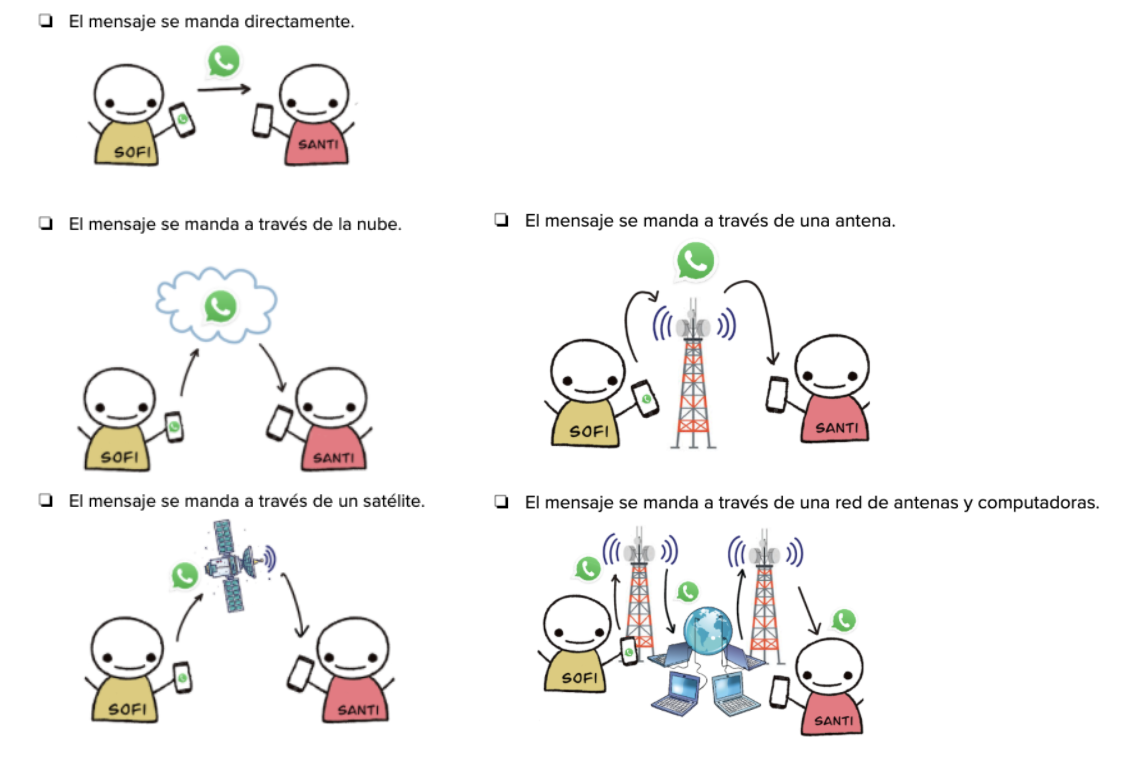
\includegraphics[width=0.90\textwidth]{images/1.png}
    \caption{Posibles opciones de respuesta para la pregunta acerca de la conectividad móvil.}
    \label{fig:cuest1}
\end{figure}

\subsection{Gratuidad de las aplicaciones en Internet}

Por último, intentamos conocer qué piensan acerca de la gratuidad de las aplicaciones en Internet: ¿por qué pueden acceder a las aplicaciones que más utilizan sin pagar? ¿De qué manera ganan dinero Facebook, YouTube, TikTok e Instagram?

La pregunta que les proponemos en la encuesta es: \textit{Muchas de las aplicaciones que conocemos se pueden usar gratuitamente, como por ejemplo Facebook, YouTube, Instagram o TikTok. ¿Por qué creés que permiten su uso sin tener que pagar?}

\section{Primera iteración: encontrando la manera de preguntar}

Al encarar la construcción del cuestionario, nuestro objetivo principal fue encontrar la manera más clara de preguntarles sobre aquello que queremos investigar.   

Al diseñar un cuestionario cerrado, los y las participantes deberán responder a solas, por lo que es muy importante que las preguntas puedan ser interpretadas y entendidas de la manera menos ambigua posible, ya que no habrá intervención nuestra al momento de realizar la actividad.

Con este fin, evaluamos que en algunos casos era necesario elaborar un “camino de preguntas”, es decir, una sucesión de preguntas que los llevara a entender la pregunta que queríamos hacer finalmente o bien, que les permitiera entrar en contexto respecto del tema para entender qué era lo que queríamos preguntarles.

\begin{figure}[h]
    \centering
    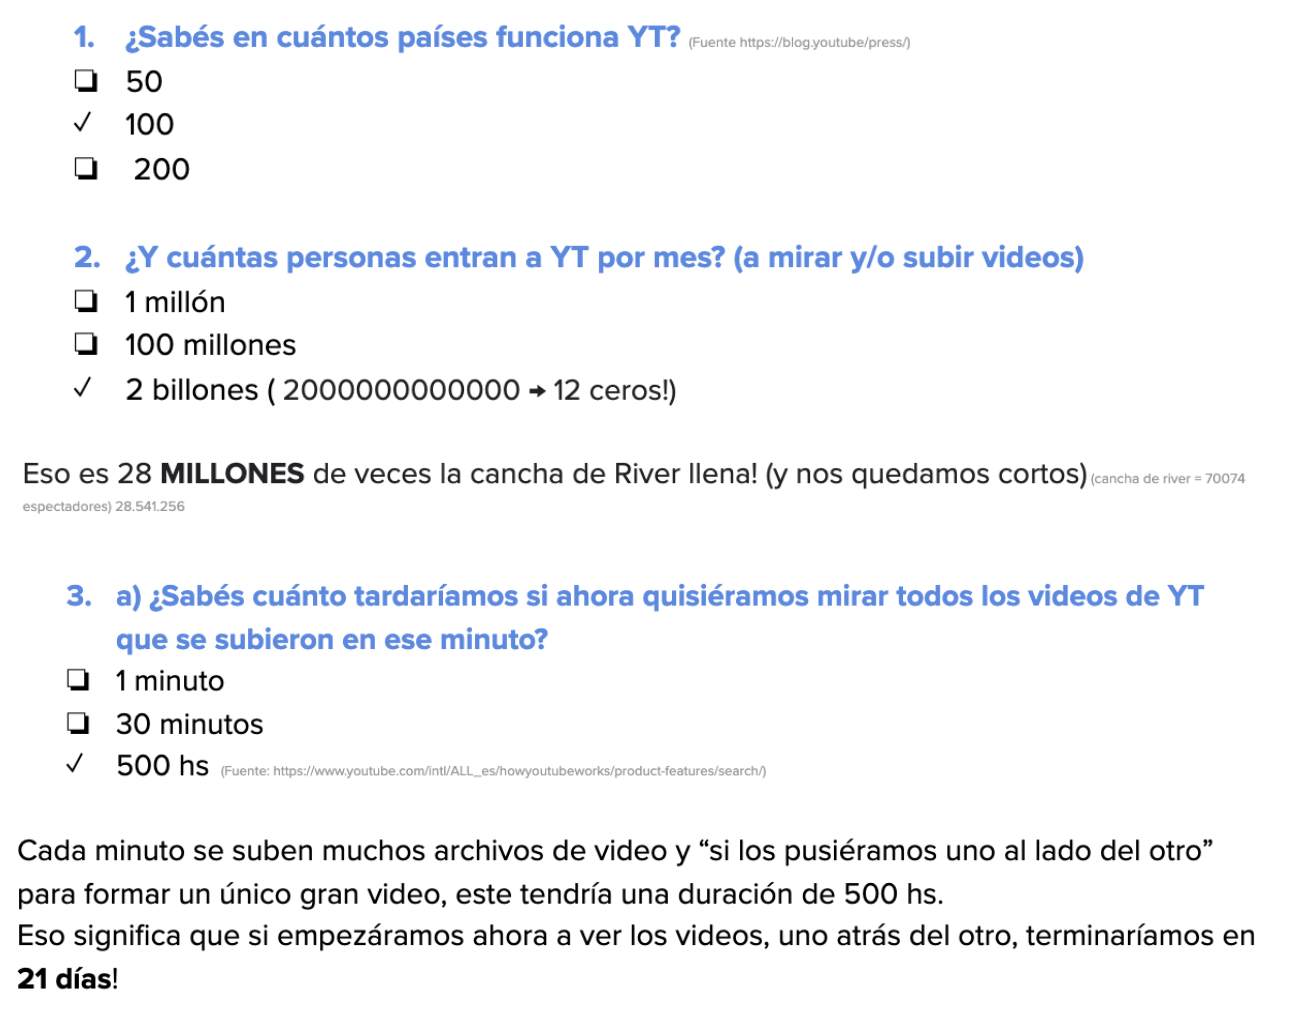
\includegraphics[width=0.75\textwidth]{images/2.png}
    \caption{Primera versión de la pregunta sobre almacenamiento de datos en YouTube, utilizando múltiples preguntas y únicamente texto.}
    \label{fig:cuest2}
\end{figure}

En la versión que se observa en la Fig \ref{fig:cuest2}, intentábamos dar a los niños y niñas una dimensión de la cantidad de datos que se almacenan en plataformas como YouTube. Sin embargo, hay que tener presente el no “guiarlos” en las preguntas, ya que no queremos “enseñarles” durante el cuestionario, o sesgar sus respuestas hacia una interpretación en particular, sino que puedan responder lo más libremente posible.

\section{Segunda iteración: refinando las preguntas}

Realizamos distintas rondas de mejoras y cambios en la encuesta hasta llegar a la versión final. En cada una de estas iteraciones, trabajamos en encontrar cuál era el equilibrio entre dar contexto a una pregunta (realizando múltiples preguntas sobre el mismo tema) y guiar demasiado a una respuesta determinada o limitar la posibilidad de responder independientemente.  

Así por ejemplo, iteramos en la pregunta anterior repensando cómo abordar la noción de los datos almacenados en YouTube y agregando imágenes, como podemos observar en la Fig \ref{fig:cuest3}.

\begin{figure}[h]
    \centering
    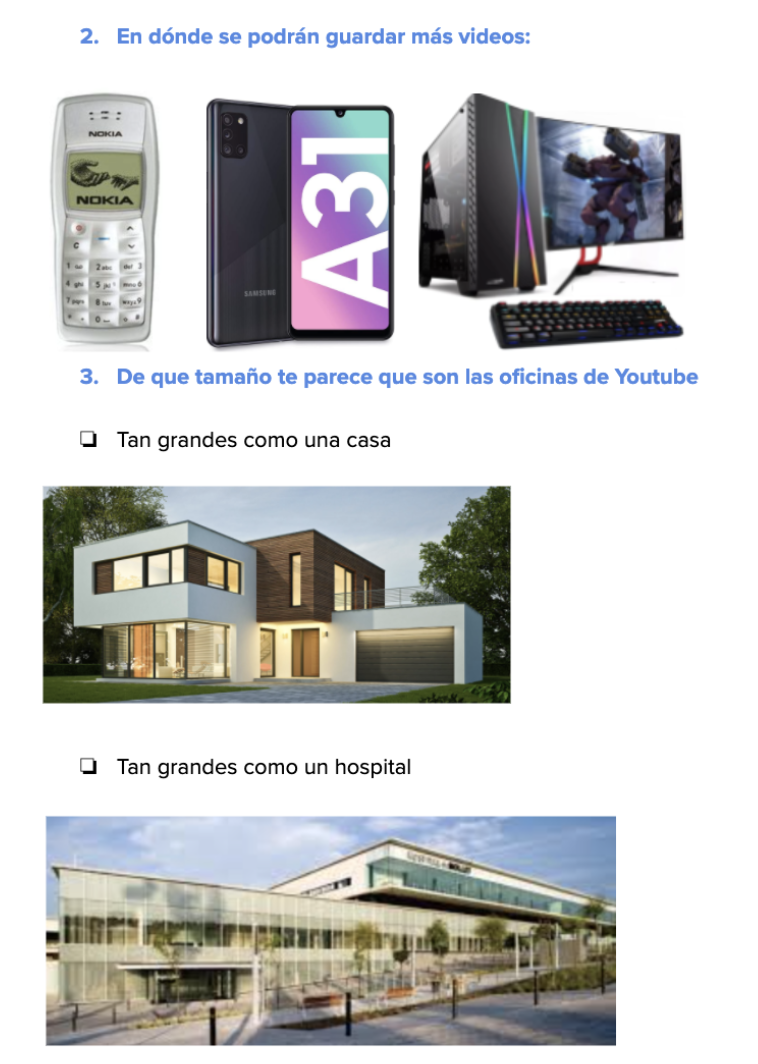
\includegraphics[width=0.5\textwidth]{images/3.png}
    \caption{Segunda versión, utilizando imágenes.}
    \label{fig:cuest3}
\end{figure}

\section{Tercera iteración: llegando a una versión más cerrada}

Ya en una tercera iteración del cuestionario, decidimos encarar la pregunta relacionada al almacenamiento de datos en YouTube de una manera más directa, pero apoyándonos en ilustraciones que nos permitieran ejemplificar las respuestas, como podemos ver en la Fig \ref{fig:cuest4}. Valiéndonos de esta ayuda visual, intentamos que el tema sea más accesible.

\begin{figure}[h]
    \centering
    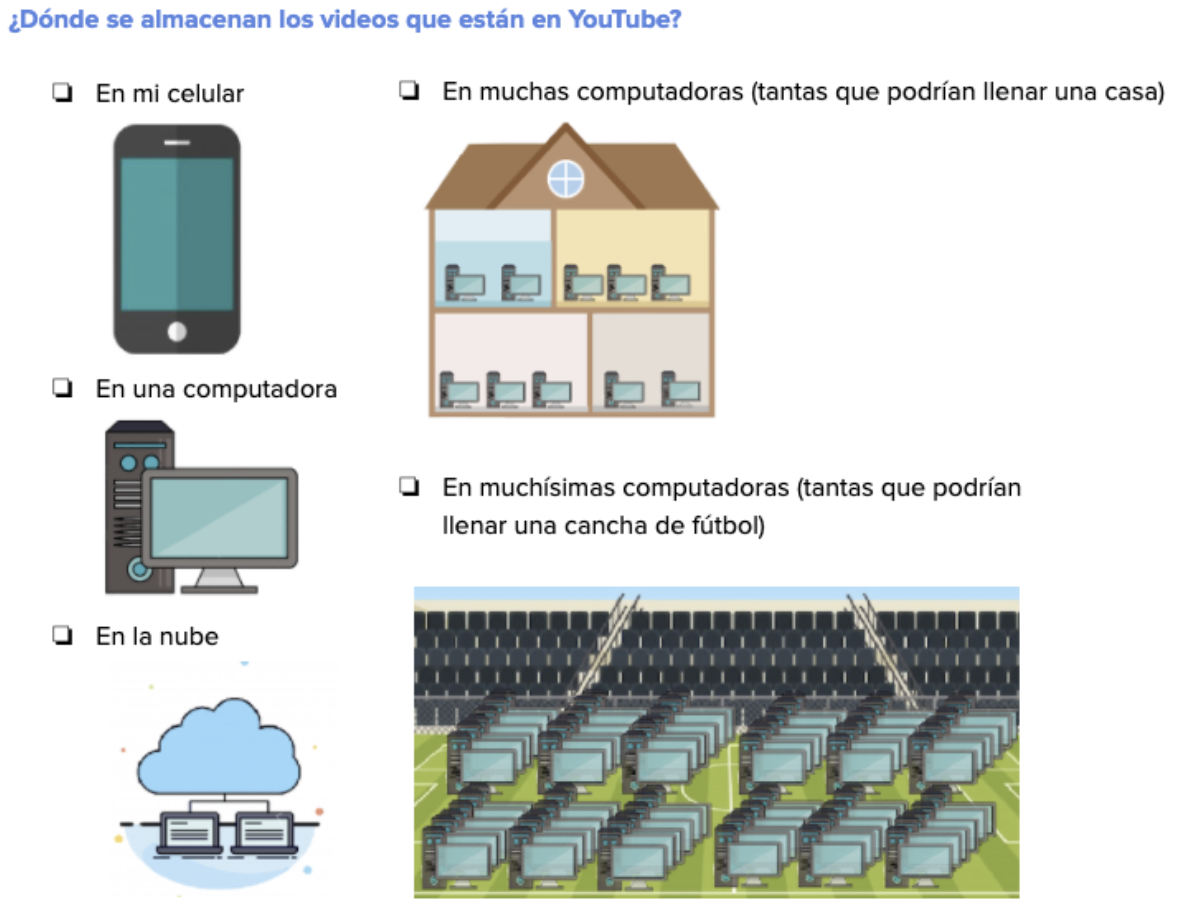
\includegraphics[width=0.8\textwidth]{images/4.png} 
    \caption{Tercera versión, utilizando ilustraciones.}
    \label{fig:cuest4}
\end{figure}

\newpage

\section{Anonimato y datos poblacionales}

Si bien la participación de los chicos y chicas en el cuestionario fue de carácter anónimo, es decir, no quedaron registrados sus datos personales de ninguna manera, agregamos una sección de preguntas poblacionales, destinadas a clasificar posteriormente la información en función de algunas variables demográficas, tales como edad y género. También les solicitamos información relativa al uso de computadoras y celulares (dónde y cuándo los utilizan, cómo aprendieron a hacerlo y cuál es el uso mayoritario que le dan a ambos dispositivos).     

Por último, recolectamos datos relacionados al contexto social de la escuela a la que asisten y a la carga académica de los alumnos en materias relacionadas a la Computación, Informática o Ciencias de la Computación para, de esta manera, tener un panorama más amplio del contexto de los niños y niñas que participan de nuestro estudio.

\section{Pruebas piloto}

Como paso previo a difundir la encuesta decidimos realizar una serie de pruebas piloto. Estas tuvieron como objetivo comprobar si las preguntas que realizamos son bien comprendidas, si las imágenes que las acompañan ayudan a clarificarlas y no generan confusiones, y si los temas son adecuados. Además, les pedimos a los participantes de estas pruebas que nos dieran su opinión respecto del cuestionario: ¿Les pareció fácil? ¿Difícil? ¿Cambiarían algo? ¿Es necesario agregar alguna opción en alguna pregunta?

Realizamos las pruebas pilotos en dos etapas. En la primera etapa entrevistamos a tres niñas y niños de alrededor de 10 años. Comenzamos teniendo una entrevista con el adulto responsable, en la que le explicamos acerca de la actividad, cómo sería realizada y del carácter anónimo de la misma. Además, le pedimos que no ofreciera su ayuda ni interviniera en ningún momento, de manera de no condicionar sus respuestas. A continuación, tuvimos una breve presentación con los chicos y chicas, en la que les explicamos el objetivo del cuestionario y les pedimos que completaran la encuesta.

Cabe destacar que, como realizamos las entrevistas en un contexto remoto, les pedimos a los tres participantes que nos compartieran su pantalla para poder ver cómo completaban la encuesta en tiempo real y, de esta manera, tratar de imitar lo más posible la presencialidad.  Esto nos proveyó de una información muy rica, ya que fuimos capaces de ver sus expresiones al leer las preguntas e identificar qué partes les eran confusas o les presentaban mayor dificultad. 

Como resultado de la primera vuelta de pruebas piloto, pudimos corroborar que las temáticas elegidas les eran conocidas y que las tecnologías indagadas eran utilizadas por ellos en su vida diaria.

También nos expresaron que en algunos casos habían tenido dificultad para entender lo que se les estaba preguntando, siendo lo más señalado la pregunta referida a la conectividad de los celulares.

A partir del \textit{feedback} recibido, decidimos reducir la cantidad de opciones que ofrecíamos como posibles respuestas, ya que nos pareció que el inconveniente radicaba en las diferencias sutiles que había entre ellas. 

\begin{figure}[h]
    \centering
    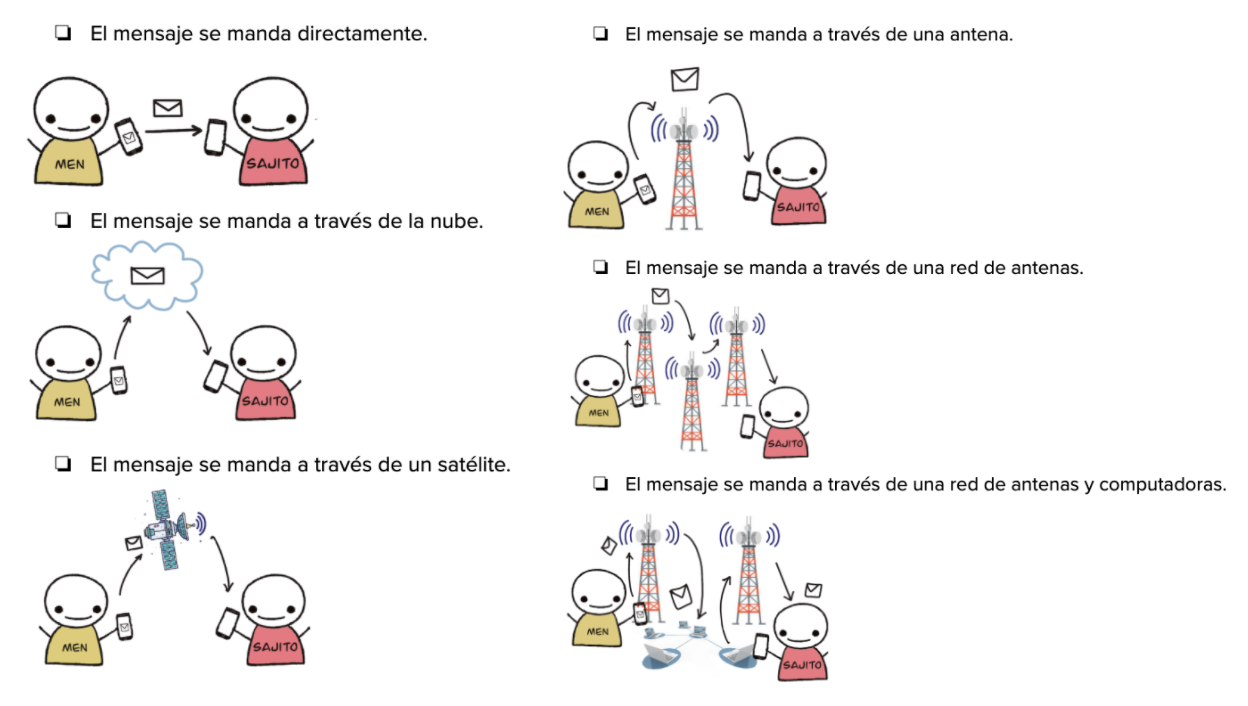
\includegraphics[width=0.8\textwidth]{images/5.png} 
    \caption{Versión inicial.}
    \label{fig:cuest5}
\end{figure}


\begin{figure}[h]
    \centering
    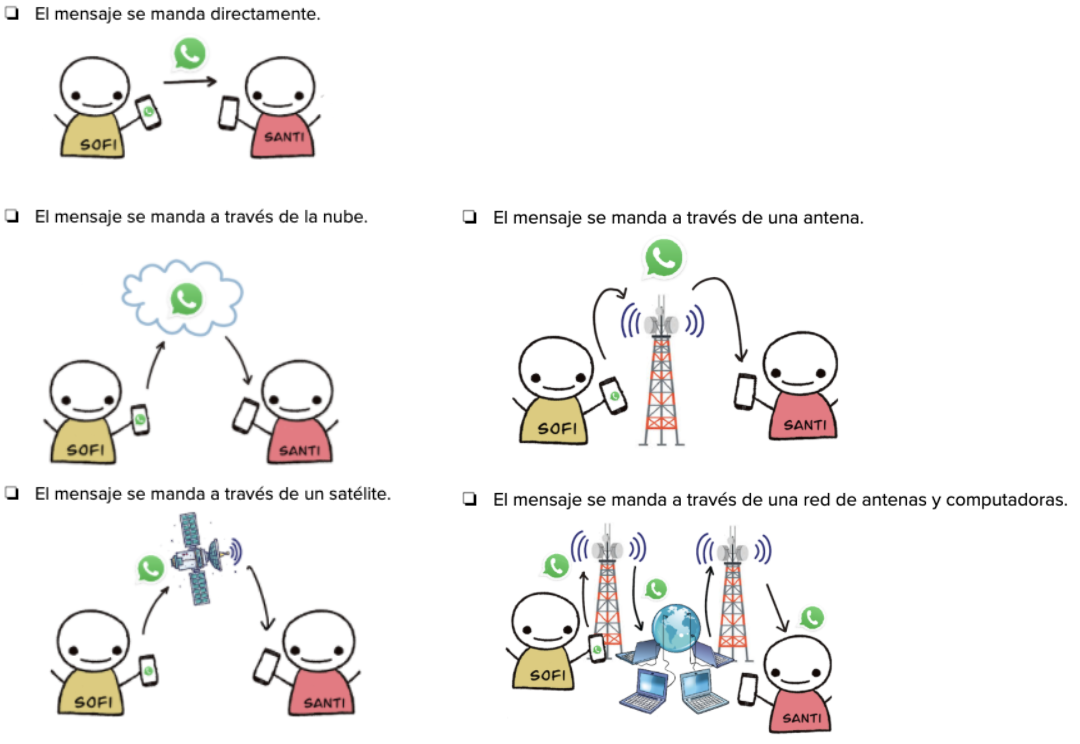
\includegraphics[width=0.7\textwidth]{images/6.png} 
    \caption{Versión final.}
    \label{fig:cuest6}
\end{figure}


En el caso de la Fig \ref{fig:cuest5} podemos ver la primera versión de la pregunta sobre conectividad donde había más opciones para elegir: una antena, múltiples antenas o antenas y computadoras. Pasamos finalmente a una versión más simplificada, como se observa en la Fig \ref{fig:cuest6}, en la que la cantidad de opciones alcanza para evaluar si los niños y niñas tiene una \textit{misconception} al respecto.

Por otro lado, aprovechamos para clarificar además el tipo del mensaje al que se refiere la pregunta (en este caso, cambiando el dibujo genérico de un sobre por el logo de WhatsApp), ya que habíamos notado que no había quedado del todo claro al tipo de mensaje al que la pregunta apuntaba, y eso había generado dudas en algunos casos. 

\newpage

Otra cuestión recurrente en las entrevistas de prueba fue que la pregunta relativa a la gratuidad de las aplicaciones en Internet no les había resultado fácil ya que tenía mucho texto para leer. Para tratar de hacerla un poco más amena, pensamos en agregar ilustraciones que acompañen las opciones. Inicialmente evaluamos utilizar ilustraciones similares a las usadas anteriormente como se observa en la Fig \ref{fig:cuest7}. 

\begin{figure}[h]
    \centering
    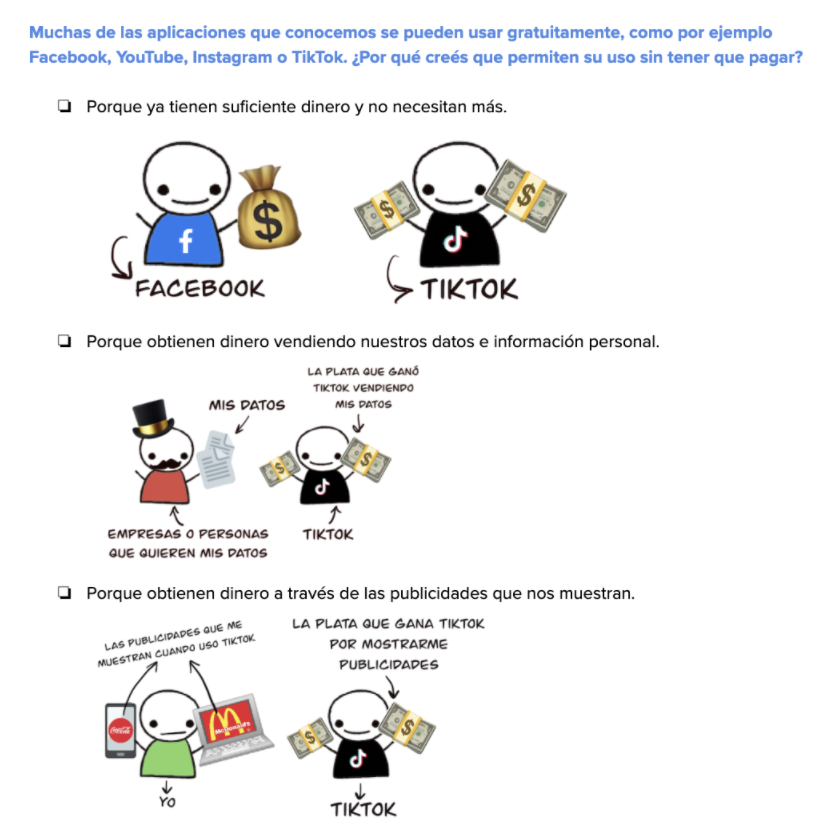
\includegraphics[width=0.7\textwidth]{images/7.png} 
    \caption{Versión inicial.}
    \label{fig:cuest7}
\end{figure}

Si bien esta opción nos parecía más simpática, decidimos ir por otro camino, ya que era posible que los dibujos sesgaran o influenciaran la respuesta. Por este motivo terminamos utilizando imágenes de textos acompañados por emojis, como podemos ver en la Fig \ref{fig:cuest8}, que facilitan la interpretación de las opciones pero que tienen menor impacto visual.

\begin{figure}[h]
    \centering
    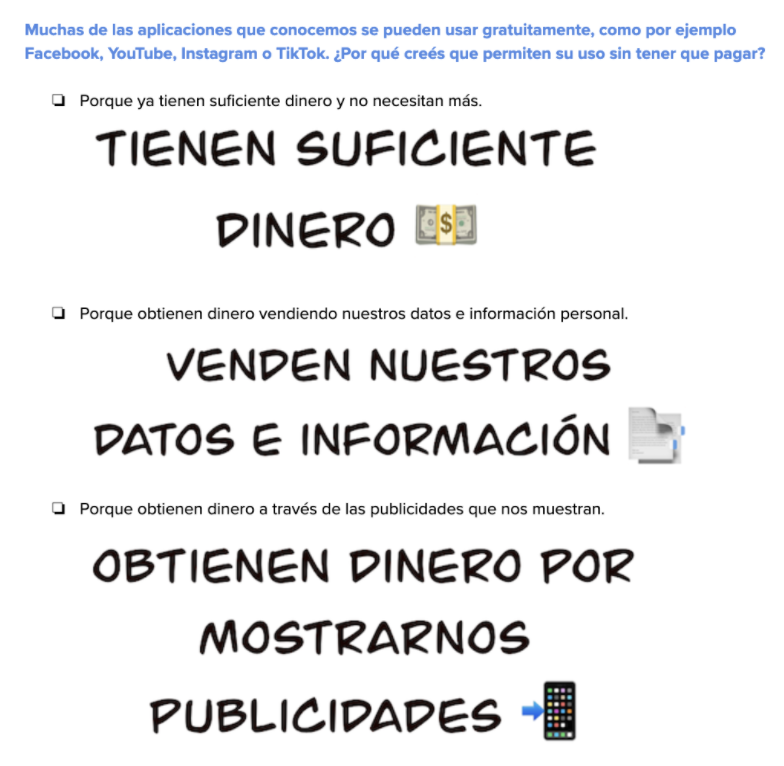
\includegraphics[width=0.6\textwidth]{images/8.png} 
    \caption{Versión final.}
    \label{fig:cuest8}
\end{figure}

Por último, agregamos a todas las preguntas la opción “No sé” ya que nos dimos cuenta en las pruebas piloto que a veces los chicos y chicas respondían cualquiera de las opciones cuando no entendían la pregunta o no conocían sobre el tema. De esta manera, les permitimos tener otra posibilidad de respuesta ante estos casos.

Tras terminar estos cambios, realizamos una segunda etapa de entrevistas y pudimos corroborar que las dificultades planteadas anteriormente se atenuaron, con lo que dimos por concluida la etapa del diseño del cuestionario. La versión final del mismo se encuentra disponible en el \autoref{chap:anexo}. 
